\chapter{LaTeX examples}

\section{Figures and images}
Lorem ipsum dolor sit amet, consectetur adipiscing elit. Sed nec ligula vel
ante placerat dapibus. Vestibulum non sollicitudin tellus. Sed varius
vestibulum libero, in euismod purus dapibus sed. Pellentesque malesuada, urna
nec lobortis egestas, felis elit varius ante, in tincidunt nunc metus id diam.
Morbi sagittis velit at ipsum sodales, in tempor nulla volutpat. Integer a
neque eros. In ipsum erat, pellentesque at dapibus eget, pretium sed risus.
Vivamus quis metus vitae felis tempus vulputate eget id lacus. Aenean sit amet
gravida quam, et ornare erat. Praesent ullamcorper mattis dolor, non interdum
orci aliquam a. In tincidunt semper lectus. Duis quis mi ac felis vehicula
mollis. Fusce molestie arcu urna, a tempor turpis mattis nec. Aenean in massa a
risus euismod aliquet vel non libero.

\subsection{One figure}

\begin{figure}[h]
    \centering
    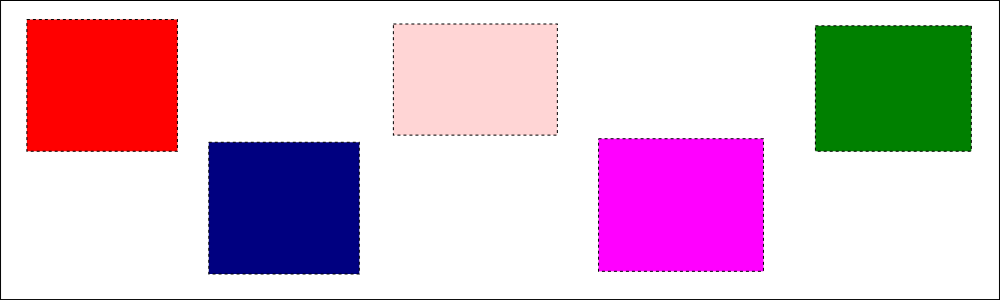
\includegraphics[width=\textwidth]{figures/test_image}
    \caption{Test Image}
    \label{fig:test_image}
\end{figure}

Aenean luctus quam ut neque viverra, quis vulputate mi hendrerit. Nunc id leo
id dui semper blandit. Nulla orci ligula, posuere non lacinia non, aliquet non
massa. Quisque gravida in mi eget volutpat. Fusce convallis felis sed dolor
ornare rhoncus. Nullam sed lacus id lectus venenatis pulvinar eget ac arcu. Sed
id turpis in leo sollicitudin euismod nec ac enim. Nunc vitae lacus lectus.
Class aptent taciti sociosqu ad litora torquent per conubia nostra, per
inceptos himenaeos. Figure \ref{fig:test_image}, Integer gravida, orci vitae
viverra ullamcorper, quam libero tempor est, non gravida magna eros id augue.
In lobortis et est auctor congue. Aliquam sed ante lacus. Vestibulum aliquam
elit eget elementum facilisis. Quisque eget felis eu leo pharetra pharetra.

\subsection{Two sub-figures}
Nulla at purus volutpat, accumsan arcu eget, commodo felis. Cras consequat
risus at rhoncus pellentesque. Aliquam tempor sodales purus in sodales. Sed ut
augue lobortis, mattis felis a, ultricies ante. Pellentesque ac tristique
ipsum, aliquet fermentum ipsum. Sed vel elit sed odio vestibulum semper id eget
enim. Nulla sed hendrerit tortor. Aliquam quam nisl, tempor ut nisl vel,
tristique facilisis libero. Suspendisse id rutrum ante. Duis sed luctus sapien.
Nullam sed quam justo.
\begin{figure}[h]
    \begin{subfigure}[b]{0.5\linewidth}
        \centering
            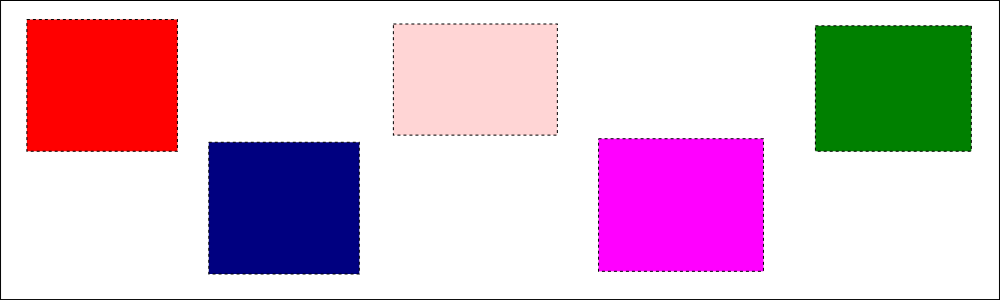
\includegraphics[width=0.9\textwidth]{figures/test_image}
            \caption{This is the caption of Sub-figure 11}
            \label{fig:subfig11}
            \end{subfigure}%
        \begin{subfigure}[b]{.5\linewidth}
            \centering
            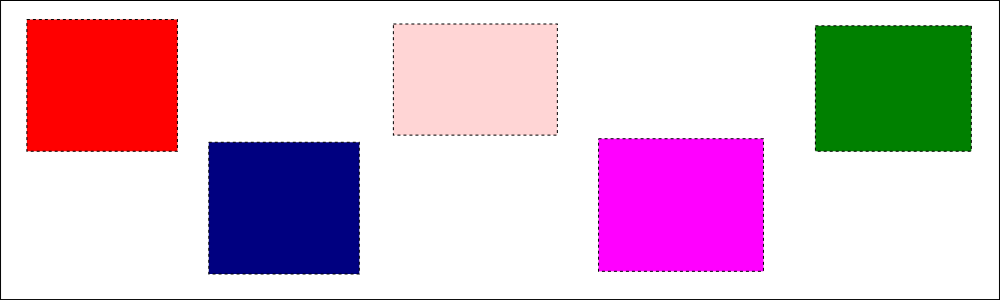
\includegraphics[width=0.9\textwidth]{figures/test_image}
            \caption{This is the caption of Sub-figure 12}
            \label{fig:subfig12}
        \end{subfigure}
    \caption{Two sub-figures}
\label{fig:sub-figures2}
\end{figure}

\subsection{Three figures together on a seperate page for floats}
Nulla at purus volutpat, accumsan arcu eget, commodo felis. Cras consequat
risus at rhoncus pellentesque. Aliquam tempor sodales purus in sodales. Sed ut
augue lobortis, mattis felis a, ultricies ante. Pellentesque ac tristique
ipsum, aliquet fermentum ipsum. Sed vel elit sed odio vestibulum semper id eget
enim. Nulla sed hendrerit tortor. Aliquam quam nisl, tempor ut nisl vel,
tristique facilisis libero. Suspendisse id rutrum ante. Duis sed luctus sapien.
Nullam sed quam justo.

\begin{figure}[p]
    \centering
    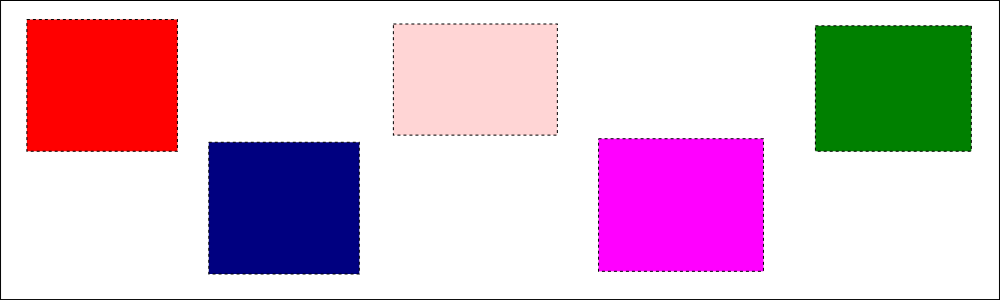
\includegraphics[width=\textwidth]{figures/test_image}
    \caption{Test Image 3}
    \label{fig:test_image3}
\end{figure}

\begin{figure}[p]
    \centering
    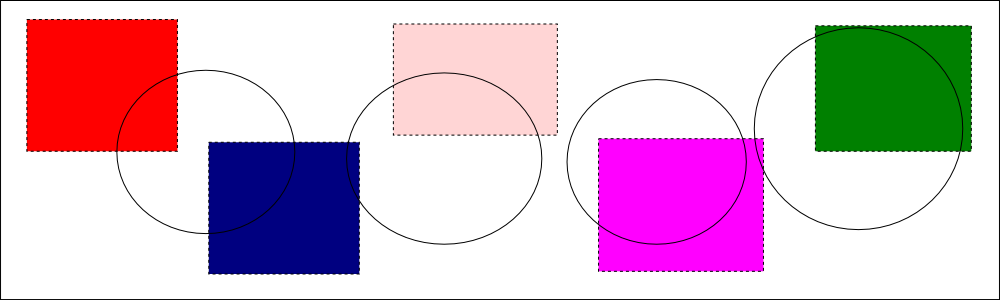
\includegraphics[width=\textwidth]{figures/test_image2}
    \caption{Test Image 4}
    \label{fig:test_image4}
\end{figure}

\begin{figure}[p]
    \centering
    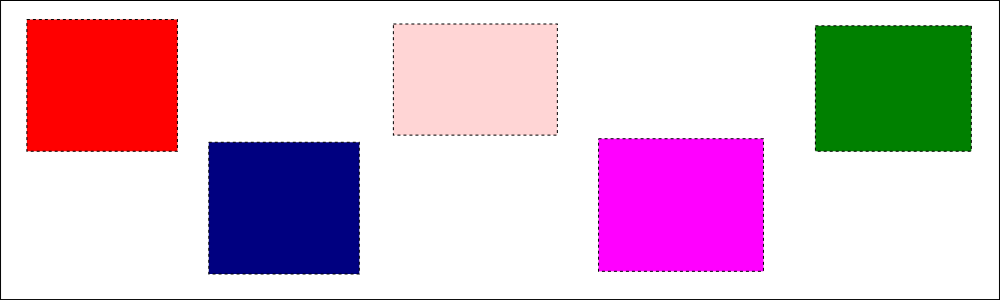
\includegraphics[width=\textwidth]{figures/test_image}
    \caption{Test Image 5}
    \label{fig:test_image5}
\end{figure}

% For more information about tables go to
% https://en.wikibooks.org/wiki/LaTeX/Tables
\section{Tables}
\subsection{One table}
Table \ref{tab:testtab2}, Aenean luctus quam ut neque viverra, quis vulputate
mi hendrerit. Nunc id leo id dui semper blandit. Nulla orci ligula, posuere non
lacinia non, aliquet non massa. Quisque gravida in mi eget volutpat. Fusce
convallis felis sed dolor ornare rhoncus. Nullam sed lacus id lectus venenatis
pulvinar eget ac arcu. Sed id turpis in leo sollicitudin euismod nec ac enim.
Nunc vitae lacus lectus.  Class aptent taciti sociosqu ad litora torquent per
conubia nostra, per inceptos himenaeos. Integer gravida, orci vitae viverra
ullamcorper, quam libero tempor est, non gravida magna eros id augue. In
lobortis et est auctor congue. Aliquam sed ante lacus. Vestibulum aliquam elit
eget elementum facilisis. Quisque eget felis eu leo pharetra pharetra.

\begin{table}[!ht]
  \centering
  \begin{tabular}{l*{6}{c}r}
      Team              & P & W & D & L & F  & A & Pts \\
      \hline
      Manchester United & 6 & 4 & 0 & 2 & 10 & 5 & 12  \\
      Celtic            & 6 & 3 & 0 & 3 &  8 & 9 &  9  \\
      Benfica           & 6 & 2 & 1 & 3 &  7 & 8 &  7  \\
      FC Copenhagen     & 6 & 2 & 1 & 3 &  5 & 8 &  7  \\
  \end{tabular}
  \caption{A floating test table.}
  \label{tab:testtab1}
\end{table}

\subsection{Two tables next to each other}
Some references to the tables on the next page, Table \ref{tab:testtab3} and
Table \ref{tab:testtab4} are sub-tables of Table \ref{tab:testtab2}. Aenean
luctus quam ut neque viverra, quis vulputate mi hendrerit. Nunc id leo id dui
semper blandit. Nulla orci ligula, posuere non lacinia non, aliquet non massa.
Quisque gravida in mi eget volutpat. Fusce convallis felis sed dolor ornare
rhoncus.

\begin{table}[!htb]
    \begin{subtable}{.5\linewidth}
      \centering
        \begin{tabular}{|r|l|}
            \hline
            7C0 & hexadecimal \\
            3700 & octal \\ \cline{2-2}
            11111000000 & binary \\
            \hline \hline
            1984 & decimal \\
            \hline
        \end{tabular}
        \caption{Caption for the first sub-table}
        \label{tab:testtab3}
    \end{subtable}%
    \begin{subtable}{.5\linewidth}
      \centering
        \begin{tabular}{|r|l|}
            \hline
            7C0 & hexadecimal \\
            3700 & octal \\ \cline{2-2}
            11111000000 & binary \\
            \hline \hline
            1984 & decimal \\
            \hline
        \end{tabular}
        \caption{Caption for the second sub-table}
        \label{tab:testtab4}
    \end{subtable}
    \caption{Caption for both tables}
    \label{tab:testtab2}
\end{table}

\subsection{One table with fixed column width}
Aenean luctus quam ut neque viverra, quis vulputate mi hendrerit. Nunc id leo
id dui semper blandit. Nulla orci ligula, posuere non lacinia non, aliquet non
massa. Quisque gravida in mi eget volutpat. Fusce convallis felis sed dolor
ornare rhoncus. Nullam sed lacus id lectus venenatis pulvinar eget ac arcu. Sed
id turpis in leo sollicitudin euismod nec ac enim. Nunc vitae lacus lectus.
Class aptent taciti sociosqu ad litora torquent per conubia nostra, per
inceptos himenaeos. Integer gravida, orci vitae viverra ullamcorper, quam
libero tempor est, non gravida magna eros id augue. In lobortis et est auctor
congue. Aliquam sed ante lacus. Vestibulum aliquam elit eget elementum
facilisis. Quisque eget felis eu leo pharetra pharetra.

\begin{table}[!ht]
  \centering
    \begin{tabular}{ | l | l | l | p{5cm} |}
    \hline
    Day & Min Temp & Max Temp & Summary \\ \hline
    Monday & 11C & 22C & A clear day with lots of sunshine.
    However, the strong breeze will bring down the temperatures. \\ \hline
    Tuesday & 9C & 19C & Cloudy with rain, across many northern regions. Clear spells
    across most of Scotland and Northern Ireland,
    but rain reaching the far northwest. \\ \hline
    Wednesday & 10C & 21C & Rain will still linger for the morning.
    Conditions will improve by early afternoon and continue
    throughout the evening. \\
    \hline
    \end{tabular}
  \caption{A floating test table with fixed column width.}
  \label{tab:testtab6}
\end{table}
